% Lecture for ph2a Caltech 2017: Vibrations and Waves
\documentclass[pdf,hideothersubsections]{beamer}
\usepackage{beamerthemeshadow}
\mode<presentation>
  {
    \usefonttheme{structuresmallcapsserif}
    \usetheme{CambridgeUS}
    \usecolortheme{seahorse}
    %\useinnertheme{circles}
%    \useoutertheme{tree}
  }

\usepackage{svg}
\usepackage{xmpmulti}

\usepackage{hyperref}
\hypersetup{
    pdffitwindow=true,     % window fit to page when opened
    colorlinks=true,       % false: boxed links; true: colored links
    linkcolor=orange,          % color of internal links (change box color with linkbordercolor)
    citecolor=green,        % color of links to bibliography
    filecolor=magenta,      % color of file links
    urlcolor=blue,           % color of external links
   pdfstartview={Fit}
}

% Fonts/encoding
\renewcommand{\UrlFont}{\tiny}
\usepackage[utf8]{inputenc}
\usepackage[T1]{fontenc}
%\usepackage[sc,medium,raggedright]{titlesec}
\usepackage{newtxmath}
%\usepackage{libertine}
\usepackage[osf]{ebgaramond}

\graphicspath{{Figures/}}

\begin{document}
\title{Coupled Oscillators}  
\author{Caltech: ph2a}
\date{10 - Oct - 2017}
%\logo{
\includegraphics[height=0.5cm]{../caltech_logo.png}}

\frame{\titlepage} 

\frame{\frametitle{Table of contents}\tableofcontents} 

\setbeamerfont{footnote}{size=\tiny}

\section{Previous Summary}
\begin{frame}
\frametitle{Recently}
\begin{itemize}
\item Complex Solutions to harmonic oscillator
\item Driven Oscillators (Wine Glass demo...)
\item Quality Factor
\item Ombuds Meeting
\end{itemize}
\end{frame}


\section{Harmony and a Wine Glass}
\begin{frame}
\frametitle{Resonant Ampification}
How much amplification do we get from a resonant system?
\pause
\begin{enumerate}
\item For a usual free mass, driven sinusoidally, $F = m a \implies x = - (F_0/m) / \omega^2$
\pause
\item For a resonant mass-spring, we have instead: $A =
  \frac{F_0/m}{\omega_0^2 + i \omega \frac{b}{m} - \omega^2}$
\pause
\item At the resonant frequency, $\omega = \omega_0$, so $A =
  \frac{F_0/m}{i \omega \frac{b}{m}}$ or, substituting our expression
  for Q,...
\pause
\item we see the amplification factor is just $Q$:  $A = -i Q \frac{F_0/m}{w_0^2}$

\end{enumerate}

\end{frame}

\begin{frame}
\frametitle{The Quality Factor: II}

\begin{columns}
\begin{column}{0.4\textwidth}
\pause
\begin{block}{Definition II:}
\centering
$Q \equiv \frac{\omega_R}{\Delta \omega}$
\end{block}
\pause
where $\Delta \omega$ is defined as the width of the peak at the
points at which: \\
\centering
$|A(\omega)|^2 = \frac{1}{2} |A_{max}|^2$

\end{column}

\pause
\begin{column}{0.6\textwidth}
\centering
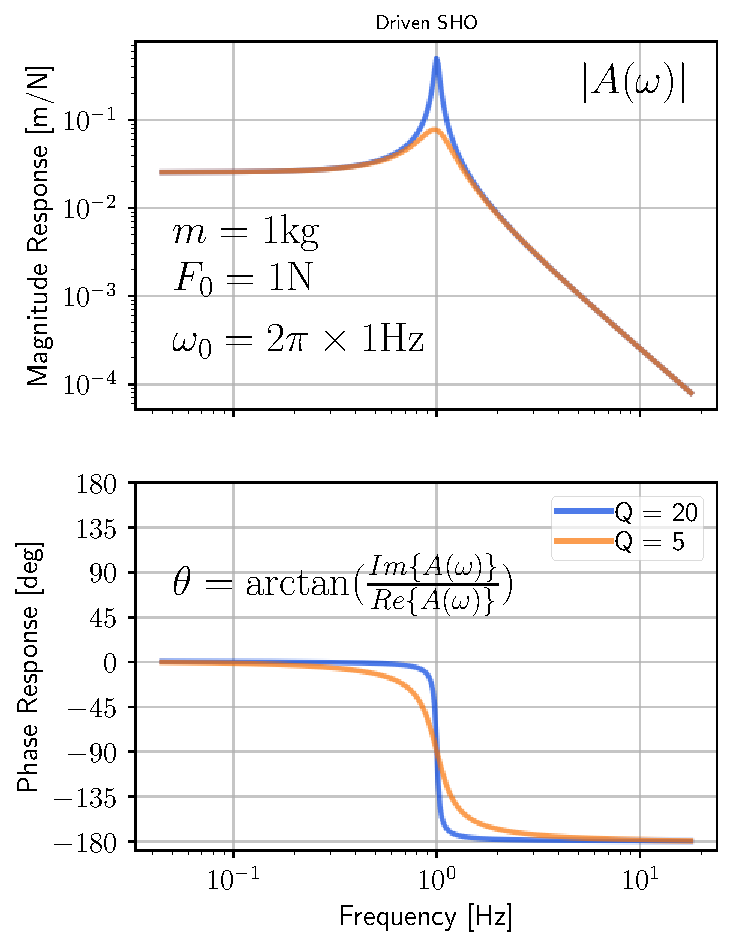
\includegraphics[width=0.8\textwidth]{DrivenSHO.pdf}

\end{column}
\end{columns}
\pause
DEMO: Wine glass with a loudspeaker, strobe light, and \emph{laser}.
\end{frame}



\section{Coupled Oscillator}
\begin{frame}
\frametitle{Coupled Oscillators: Overview}
\pause
\begin{enumerate}
\item For free vibrations, $m \ddot{x} + b \dot{x} + k x = 0$.
\pause
\item In a coupled systems, there can be several springs and several
  masses with many inter-connections.
\pause
\item Also applies in the case of complicated circuits.
\pause
\item Matrix methods are very handy in solving systems of coupled
  differential equations.
\end{enumerate}
\end{frame}

\subsection{Examples}
\begin{frame}
\frametitle{Examples}

\begin{itemize}
\item 2 masses, 3 springs (Airtrack Demo)
\pause
\item 2 Pendula coupled by a weak spring

\end{itemize}


\end{frame}


% \begin{frame}
% \frametitle{More Examples}

% \begin{table}
% \centering
%     \resizebox{\columnwidth}{!}{%
%     \begin{tabular}{|l|c|r|}
%       \hline
%     Item Name                     & Frequency (Hz)  & Quality Factor \\ \hline
%     Strings                       & 10       & 0.5      \\
%     Big Bang                & 330      & 1500     \\
%    The Sun                   &         &          \\
%   Lasers                         &         &          \\
%    Mass on Track (w/ magnetic damping)   &         &          \\
%   Suspension Bridges (e.g. Golden Gate)  &         &           \\
%   Ionosphere (Schumann resonances)        & 8-30   & 3-5       \\
%     Stop Sign (hit with a rubber mallet) & 200      & 1000     \\
%     ${}_0S_0$ Dilational Mode of the Earth     & 0.0008   & 3000     \\
%     75 mm silicon wafer                  & 800      & 50,000   \\
%     Quartz Crystal Resonator             & 10$^6$   & $10^4$\,--\,$10^6$ \\
%     Large, High Purity Glass             & 3000     & 10$^8$   \\ \hline
%     \end{tabular}}
% \end{table}

% \end{frame}


\subsection{Equations of Motion}
\begin{frame}
\frametitle{Two Masses + Three Springs}
\begin{columns}

  \begin{column}{0.5\textwidth}
\pause
    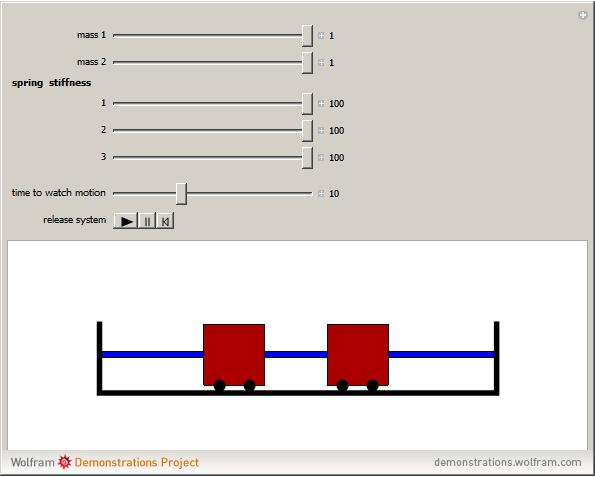
\includegraphics[width=0.85\textwidth]{2masses3springs-cdf.jpg}
\url{http://demonstrations.wolfram.com/MotionOfTwoMassesConnectedBySprings/}
  \end{column}

  \begin{column}{0.5\textwidth}
    \pause
    Forces on Mass 1:
    \begin{equation}
      F_1 = m \ddot{x_1} = -k x_1 + k (x_2 - x_1)
    \end{equation}
    \pause
    Forces on Mass 2:
    \begin{equation}
      F_2 = m \ddot{x_2} = -k x_2 - k (x_2 - x_1)
    \end{equation}
    \pause
    2 Eqs \& 2 Unknowns:
    \begin{align}
      m \ddot{x_1} + 2 k x_1 - k x_2 &= 0 \\
      m \ddot{x_2} + 2 k x_2 - k x_1 &= 0
    \end{align}
  \end{column}

\end{columns}
\end{frame}



\begin{frame}
\frametitle{Two Masses + Three Springs}
    \pause
\begin{enumerate}
\item For SHO, we guessed $\tilde{x} = A e^{i (\omega t + \phi_0)}$
\pause
\item For CHO, we use $\tilde{x_1} = A_1 e^{i \omega t}$ and
  $\tilde{x_2} = A_2 e^{i \omega t}$; assuming $A_1$ and $A_2$ are complex.
\pause
\item Plugging into Eqs. 3 \& 4, we get: \\
\begin{align*}
\Big[ -\omega^2 A_1 + 2 \frac{k}{m}A_1 - \frac{k}{m}A_2 \Big] e^{i
  \omega t} &= 0 \\
\Big[ -\omega^2 A_2 + 2 \frac{k}{m}A_2 - \frac{k}{m}A_1 \Big] e^{i
  \omega t} &= 0
\end{align*}
\pause
\item Divide both sides by $e^{i \omega t}$ and using $\omega_0^2 =
  k/m$, we get:
\pause
\begin{align*}
\Big[ -\omega^2 A_1 + 2 \omega_0^2 A_1 - \omega_0^2 A_2 \Big] &= 0 \\
\Big[ -\omega^2 A_2 + 2 \omega_0^2 A_2 - \omega_0^2 A_1 \Big] &= 0
\end{align*}

\end{enumerate}
\end{frame}

\section{Eigenfrequencies}
\begin{frame}
\frametitle{Matrix Methods: Eigenvalues}
\pause
Rewrite in matrix form to allow using linear algebra: \\
\[
\begin{bmatrix}
-\omega^2 + 2 \omega_0^2 & -\omega_0^2 \\
-\omega_0^2 & -\omega^2 + 2 \omega_0^2
\end{bmatrix}
\begin{bmatrix}
A_1 \\
A_2
\end{bmatrix}
=
\begin{bmatrix}
0 \\
0
\end{bmatrix}
\]
\pause
Equivalent to setting the determinant equal to zero:
\[
\begin{vmatrix}
-\omega^2 + 2 \omega_0^2 & -\omega_0^2 \\
-\omega_0^2 & -\omega^2 + 2 \omega_0^2
\end{vmatrix}
= 0
\]
\pause
which gives us the following quadratic equation:
\pause
$(-\omega^2 + 2 \omega_0^2)^2 -\omega_0^4 = 0$ \\
\pause
and solving for $\omega$, we have
\centering
\pause
$\omega^2 = 2 \omega_0^2 \pm \omega_0^2$ \\
\pause
so $\omega = (\omega_0, \sqrt{3} \omega_0)$

\end{frame}










\section{Eigenmodes}
\begin{frame}
\frametitle{Eigen (Normal) Modes}
\pause
Plugging the eigenfrequencies back into our equations, we get:
\pause
\begin{align}
\omega = \omega_0 :  -\omega_0^2 + 2 \omega_0^2 A_1 - \omega_0^2 A_2 &=
0 \implies A_1 = A_2\\
\omega = \sqrt{3} \omega_0 :  -3 \omega_0^2 + 2 \omega_0^2 A_1 - \omega_0^2 A_2 &=
0 \implies A_1 = - A_2
\end{align}
\pause
These are the \emph{symmetric} and \emph{anti-symmetric} solutions, respectively.


\end{frame}


% \section{Beats}
% \begin{frame}
% \frametitle{Beats: Examples}
% \end{frame}




\section{Summary}
\begin{frame}
\frametitle{Properties of Eigenmodes}
\begin{enumerate}
\pause
\item $\omega_{1,i}=\omega_{2,i}=\omega_i$~(for the i$^{th}$ mode)
\pause
\item $A_{1,i}, A_{2,i} \ne f(t)$; i.e. amplitudes are constant
\pause
\item A's are constant, so the relative phases of the modes are
  constant
\pause
\item \underline{Stable}: w/o friction the oscillations go on forever
\pause
\item \textbf{Complete}: Any motion can be decomposed into a sum of
  normal modes.

\end{enumerate}
\end{frame}


\end{document}

